\documentclass[12pt,letterpaper]{article}

\usepackage[utf8]{inputenc}
\usepackage[spanish]{babel}
\usepackage{times}
\usepackage[left=3cm,top=2.5cm,bottom=2.5cm,right=2.5cm]{geometry}
\usepackage{graphicx}

\title{EV\_ 1\_ 2\_ OptoAclopadores\_ y\_ Relevadores  }

\author{Romero Jauregui Osvaldo, Perez de Alba Santiago Eduardo}

\begin{document}
\maketitle

\section{Introducción:}
\

Los rectificadores son un circuito destinado a convertir la corriente alterna (AC) en corriente continua (DC), los cuales son ampliamente utilizados en la industria para alimentar motores de corriente continua de alta potencia, asi como; su uso en los equipos electrodomesticos para la alimentacion de sus diferentes circuitos. El principal componente que es fundamental para diseñarlos son los diodos rectificadores
\

\section{Objetivo:}
\

El crear los circuitos dados en las hojas previas para asi poder comparar las simulaciones de las onda con la del documento.

\

\section{Marco Teorico:}
\

La conversion de AC-CD tiene importancia capital en el campo de la electronica y de la electricidad general, derivada de la necesidad de adaptar las caracteristicas de las redes en distribucion electrica (principal fuente de energia que se utiliza actualmente) a los requerimentos de un amplio abanico de receptores tales como equipos electronicos, motores de corriente continua (utilizados en regulacion de procesos y en tracción  eléctrica: metro, tranvía, trenes de cercanías, etc.
\

Desde el punto de vista de los dispositivos electronicos utilizados y las posibilidades de controlar el nivel de tension continua en la salida del rectificador, este tipo de convertidores se pueden clasificar en:
\

1.- Rectificadores no controlados.
\

2.- Rectificadores controlados.
\

Los primeros utilizan diodos como dispositivo semiconductor y permiten obtener una tension de salida con un valor medio practicamente constante, sin posibilidades de variar su amplitud de forma controlada.
\

El segundo tipo de rectificadores (controlados) utilizan tiristores como dispositivo semiconductor. Su principal caracteristica es la posibilidad de controlar a voluntad el valor medio de la tension de salida del rectificador, actuando para ello sobre el angulo de disparo de los tiristores.
\

\section{Materiales:}
\

1.- Computadora (Laptop de preferencia).
\

2.-Software interactivo Orcad (Cadence).
\
3.- Juego de hojas para seguir con la practica (previamente otorgadas por el profesor).
\

\section{Procedimiento:}
\

\subsection{Rectificador de media onda con carga inductiva:}
\

(En el procedimiento se agrego el de solo un circuito ya que los procedimientos de los demás son similares).

\

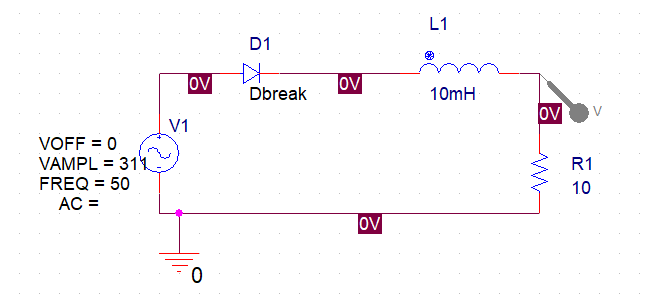
\includegraphics[width=7cm]{Circuito 1-2.png} 

\

Como se logra observar en la imagen tenemos un alternador el cual se ingresa una amplitud de 311V y una Frecuencia de 50 Hz, el cual al añadirle un diodo rectificador lo que hace que la tension de salida se anula hasta que no lo hace la corriente de carga, obteniendo como resultado el diodo rectificar polarizado.
\

\

\subsection{Rectificador monofasico en puente:}
\

Este esta constituido por un capacitor y una bobina, las cuales atenuan el rizado de la tension de salida. Mientras que por el lado alterno se incorporan R y Lr.
\

Durante el desarrollo nos encontramos con el analisis de Fourier, el cual nos ayuda con informacion sobre los armonicos y asi determinar el factor de potencia.

\

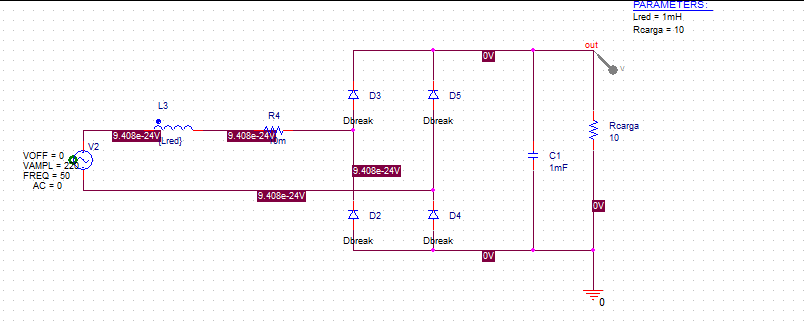
\includegraphics[width=7cm]{Circuito 1-3.png} 
\

Gracias a este circuito, al analisis de fourier, se a podido observar la distorsion de la corriente absorbida por el rectificador que repercute en un factor de potencia bajo.

\

\subsubsection{Rectificador monofasico en puente (con concepto PCC):}
\

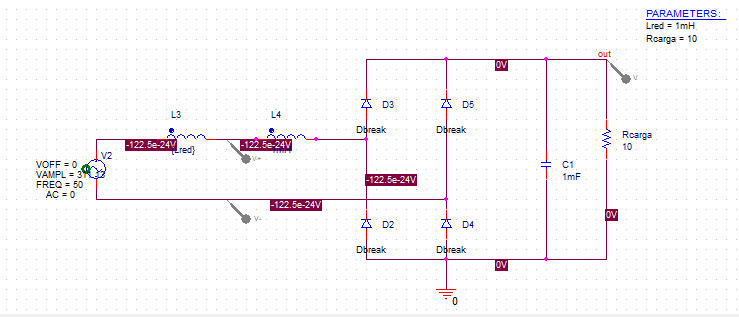
\includegraphics[width=7cm]{Circuito 1-3-2.png} 

\

Existe otro efecto sobre la red de suministro, esto se debe a que si la corriente presenta un contenido en armonicos elevado, supone que las caidas de tension producidas en la linea como consecuencia esta corriente repercutiran en una distorsion de la tension de red en el punto de conexion comun (PCC) de varios receptores.
\

Lo que se desarrolla con esta implementacio (PCC), es que la bobina 1 (L3) modeliza la inductancia de la linea de distribucion, en tanto que la bobina 2 (L4) equivale a la inductancia que existe entre el PCC y el rectificador.

\

\subsection{Rectificador monofasico duplicador de tension:}
\

Este rectificador permite obtener en la salida una tension que corresponde al doble de la que se obtiene en el Rectificador monofasico en puente.
\

Esto se obtiene gracias a que las tensiones elevadas en la etapa de continua sin necesidad de utilizar un transformador que eleve la tension de entrada del rectificador.

\

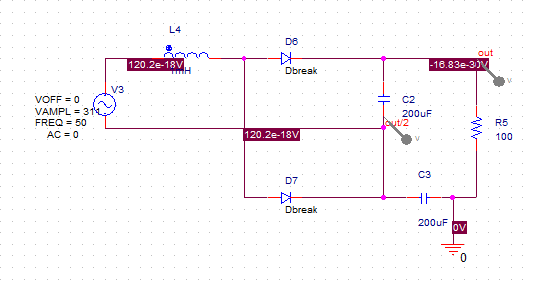
\includegraphics[width=7cm]{Circuito 1-4.png} 

\

\subsection{Efectos de los rectificadores monofasicos en lineas trifasicas:}
\

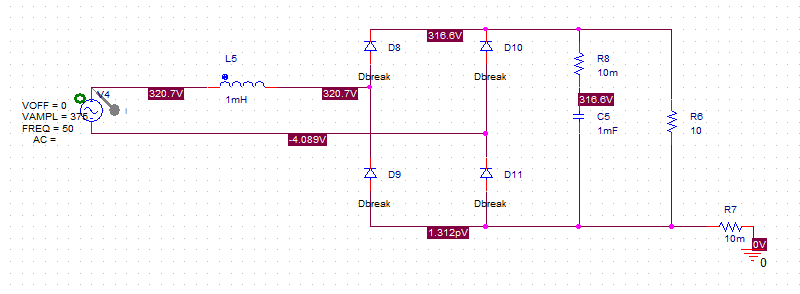
\includegraphics[width=7cm]{Circuito 1-5.png}
\

Para la realizacion de este circuito se tiene una bobina y 4 diodos los cuales en la parte superior tenemos 2 de ellos en paralelo, mientras que en la parte inferior del circuito otros 2 de igual manera en paralelo, un capacitor y dos resistencias una de ellas (R7), se coloco unicamente para evitar problemas al obtener las ondas de frecuencia.

\

\

\subsection{Rectificadores Trifasicos:}
\

Estos se implementan cuando la potencia que consuman de la red es elevado.
\

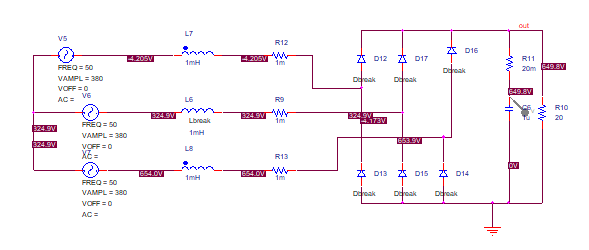
\includegraphics[width=7cm]{Circuito 1-6.png} 
\

En el circuito anterior se muestra un rectificador trifasico no controlado que es alimentado por una red de frecuencia de 50Hz y 380V. La tension de salida que tendra el rectificador es filtrado mediente la Bobina (L5,L6,L8) y el capacitor (C5).
\

El menor rizado que se obtiene en la salida es uno de los principales objetivos de los rectificadores trifasicos
\

\subsection{Efecto de las inductancias de red sobre la conmutacion de corriente: }
\

Al momento de añadir un inductor de filtro, las inductancias de la linea provoca que la conmutacion de corriente de entre los diodos del rectificador no sea al instante.
\

Esto quiere decir que cuando la tension es positiva en el diodo 1 se polariza y conduce. Por otro lado, el diodo 2 se polariza de manera inversa y permanecera bloqueado. En caso contrario, en donde la tension fuera negativa dejaria de conducir al al diodo D1, para que el diodo 2 tome su lugar.
\

La onda resultante seria casi nula durante la conduccion en el diodo D2, la funcion de la inductancia L1 es que no permite las discontinuidades bruscas en la corriente que circula por ella, por lo tanto mantiene a los diodos en conduccion por un breve periodo de tiempo.
\

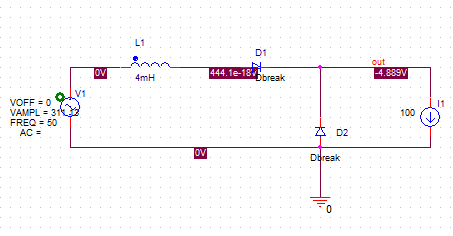
\includegraphics[width=7cm]{Circuito 1-7-1.png}
\

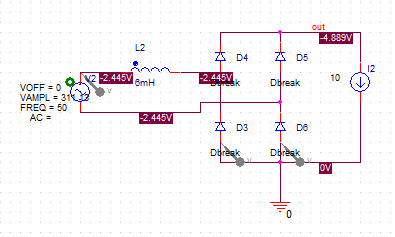
\includegraphics[width=7cm]{Circuito 1-7.png} 
\

\

\section{Resultados:}
\

\

\subsection{Rectificador de media onda con carga inductiva:}
\

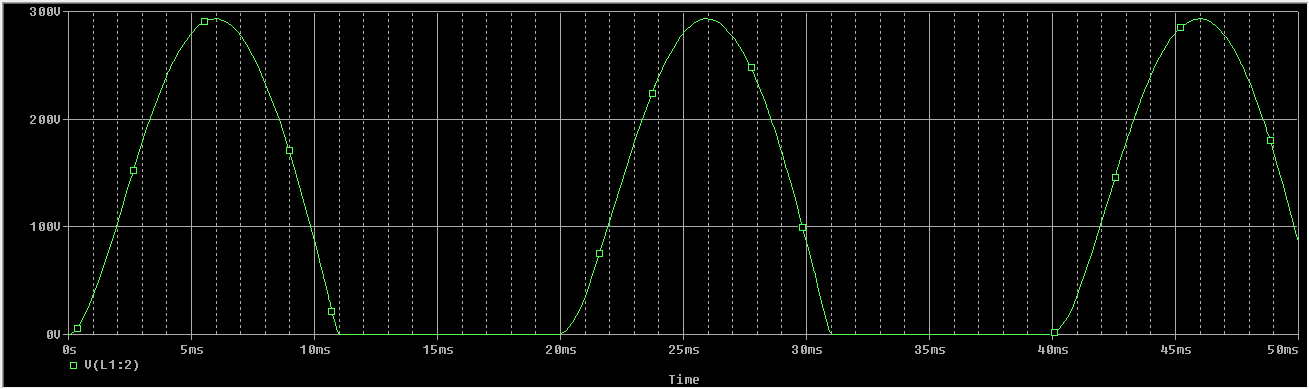
\includegraphics[width=7cm]{Resultado Circuito 1-2.png} 
\

Se puede observar que la tension de salida no se anula hasta que no lo hace la corriente de la carga, lo que significa que el diodo rectificador permanece polarizado en directo. Esto debido a la inductancia de salida que opone a las variaciones bruscas de corriente.
\

\

\subsection{Rectificador monofasico en puente:}
\

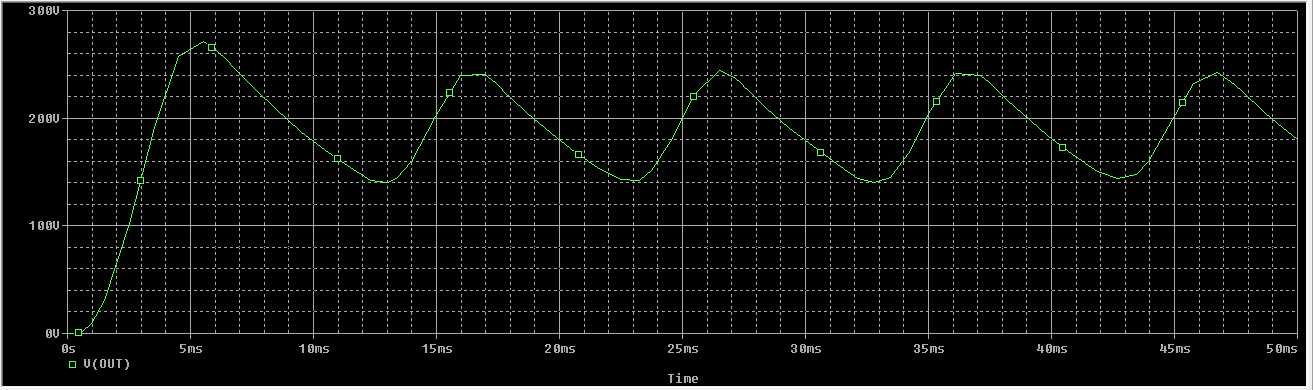
\includegraphics[width=7cm]{Resultado Circuito 1-3.png} 
\

El consumo de corriente de salida afecta al rizado. Esto debido a que el rizado disminuye a medida que lo hace el consumo de corriente, ya que el condensador es menos necesario y se descargara menos.
\
Para poder cuantificar los resultados y determinar el factor de potencia global del rectificador en condiciones de carga inicial, se utiliza el analisis de Fourier que se efectuara con el simulador.
\
Los datos recabados seran obtenidos mediante la siguiente formula:
\

\emph{Fourier}
$$ i_{Lr}(t)= C_o + \sum_{n=1}^{\infty} C_n sen(nw*t + o_n$$

\

\subsubsection{Rectificador monofasico en puente (con concepto PCC):}
\

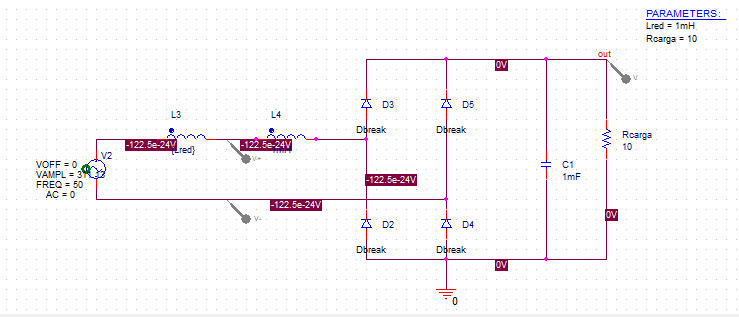
\includegraphics[width=7cm]{Circuito 1-3-2.png} 
\


Como se puede observar una tension en el punto comun de conexion que esta distorsionada a consecuencia de caidas de tension.
\
Se considera que estan recibiendo los receptores, sin embargo la calidad de las cargas fuertes no lineales, como lo es en los circuitos rectificadores.

\

\subsection{Rectificador monofasico duplicador de tension:}
\

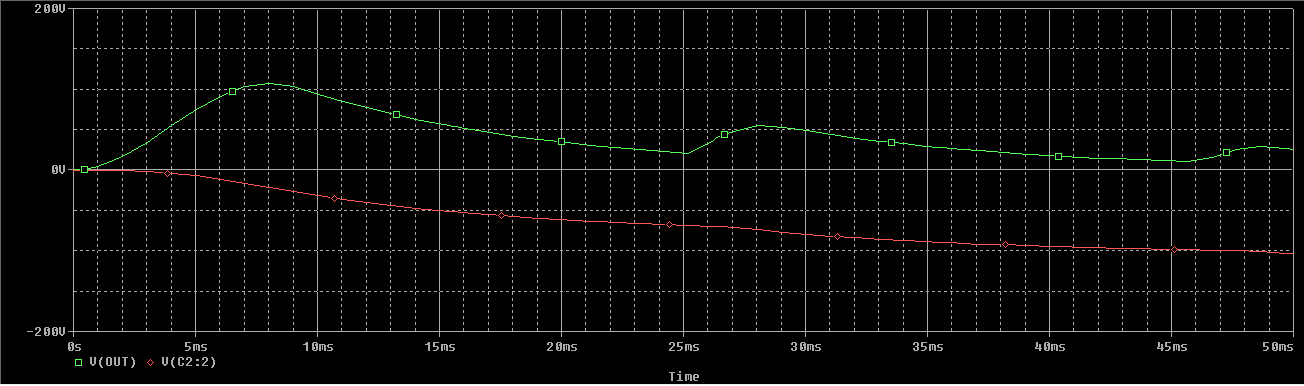
\includegraphics[width=7cm]{Resultado Circuito 1-4.png}
\

Se puede observar que el rizado pico a pico del rectificador en puente es la mitad que en el duplicador de tension, ya que la salide de (Ve) hay dos condensadores en serie, quedando asi su capacidad equivalente reducida a la mitad.
\

\

\subsection{Efectos de los rectificadores monofasicos en lineas trifasicas:}
\

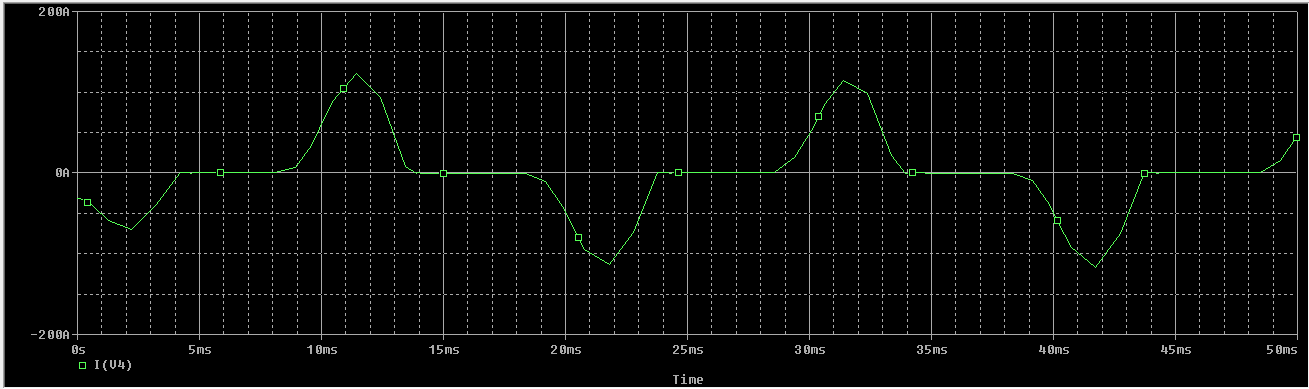
\includegraphics[width=7cm]{Resultado Circuito 1-5.png} 
\


Se puede observar que la corriente que circula por el neutro no es nula aunque los receptores monofasicos consumen la misma potencia por fase.
\

Esto quiere decir que debido a la no linealidad de los receptores, la suma de las tres corrientes de fase no es nula.

\

\

\subsection{Rectificadores Trifasicos:}
 \
 
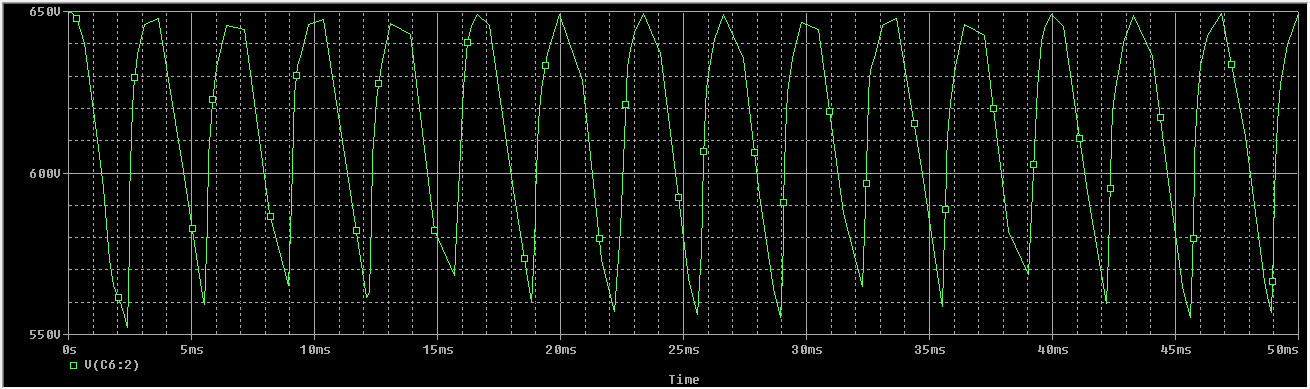
\includegraphics[width=7cm]{Resultado Circuito 1-6.png}  
 \

Como se observa en la imagen anterior, En el rizado de la tension de salida, con el valor de Cf utilizado puede medirse un valor pico a pico de 13.5v.
Esto pasa debido a que la tension de salida del rectificador trifasico sin filtrar presenta una amplitud de rizado anterior.
\

La frecuencia del rizado en el rectificador trifasico es tres veces superior.

\

\

\subsection{Efecto de las inductancias de red sobre la conmutacion de corriente: }
\

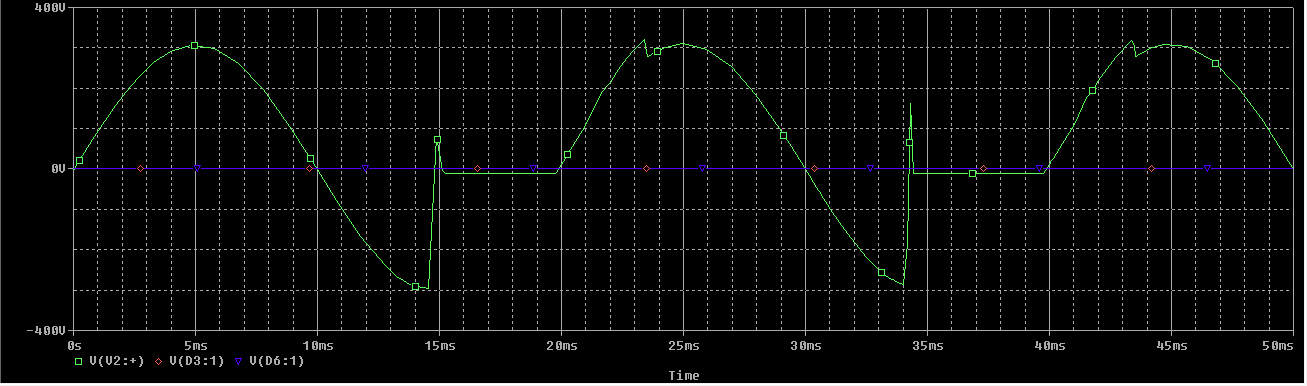
\includegraphics[width=7cm]{Resultado Circuito 1-7.png} 
\

Como se ve en la imagen anterior la inductancia no permite que haya cambios bruscos en la corriente que circula por ella, manteniendo los diodos conduciendo. Mostrando una perdida de tension debido a la conmutacion entre los diodos, debido a que la carga queda en cortocircuito durante las conmutaciones porque los cuatro diodos permanecen en conduccion.

\

\section{Conclusion:}
 \
 
 Osvaldo: \ Pese a ser un software que no habíamos utilizado con anterioridad, el uso de OrCad nos ayudo en la elaboración de nuestras simulaciones. Conforme fuimos avanzando con los distintos circuito nos fuimos dando una idea de los distintos tipos de ondas.
 \
 
 \

Santiago:\ Al desarrollar la practica pudimos observar el funcionamiento de los circuitos rectificadores, como estan conformados y cuales son sus funcionamiento, como tambien el como afecta a las ondas de frecuencia.
 



\end{document}